\documentclass[a4paper, 12pt]{report}
\usepackage[T1]{fontenc}
\usepackage[utf8]{inputenc}
\usepackage[english]{babel}
\usepackage{mathtools}
\usepackage{amsfonts}
\usepackage{amsmath}
\usepackage{mathrsfs}
\usepackage{enumitem}
\usepackage{booktabs}
\usepackage{array}
% Avoid paragraph indent
\setlength{\parindent}{0pt}
% Useful floor and ceiling functions
\DeclarePairedDelimiter{\floor}{\lfloor}{\rfloor}
\DeclarePairedDelimiter{\ceil}{\lceil}{\rceil}
% Modified margins
\usepackage[margin=2cm]{geometry}
% This avoids hypenation
\hyphenpenalty=10000
\usepackage{tikz}
\usetikzlibrary{arrows,calc,positioning,shadows,shapes}
\usepackage{graphicx}
\graphicspath{ {figs/} }
\usepackage{subfig}
\captionsetup[figure]{labelfont={bf},name={Figure},labelsep=period}
\captionsetup[table]{labelfont={bf},name={Table},labelsep=period}

\usepackage{float}


\begin{document}
	
\title{Digital Communications and Laboratory \\ First Homework}
\author{Faccin Dario, Pegoraro Jacopo}
\date{}
\maketitle

\section*{Problem 1}

\subsection*{Input signal}
The random process to simulate is:
\begin{equation}
x(k)=e^{j(2\pi f_1 k +\phi_1)} + 0.8e^{j(2\pi f_2 k +\phi_2)} + w(k)
\end{equation}
\noindent where $f_1=0.17$ and $f_2=0.78$ are the normalized frequencies of the exponential signals, $\phi_1$ and $\phi_2$ their initial phases considered as uniformly distributed in the interval $ [0,2\pi)$. The added noise $w(k)$ is a r.p. that follows a complex Gaussian distribution with zero mean and variance $\sigma_w^2$.
The simulation of this process has been carried out for $K=800$ samples of a single realization.

\subsection*{Autocorrelation estimation}

An unbiased estimate of the autocorrelation of the signal is provided by \cite{nevio<3}:
\begin{equation}
{\hat{\mathtt{r}}_x(n)}=\frac{1}{K-n} \sum_{k=n}^{K-1} x(k) x^*(k-n) \mbox{, for } n=0,1,...,K-1
\end{equation}
where $K$ is the number of samples of the realization of $x(k)$.  

A biased estimate of the autocorrelation is instead \cite{nevio<3}:
\begin{equation}
{\check{\mathtt{r}}_x(n)}=\frac{1}{K} \sum_{k=n}^{K-1} x(k)
x^*(k-n)= \Big(1-\frac{|n|}{K}\Big)\hat{\mathtt{r}}_x(n)
\end{equation}

The variance of the estimate gets larger and larger as $n$ approaches $K$. For this reason the number of samples that provide a reliable estimate ($=L$) is much lower than the length of $x(k)$. In the following analysis we will state in each method the value of $L$ used.

\subsection*{Blackman and Tukey Correlogram}
This estimator uses the autocorrelation unbiased estimation $\{{\hat{\mathtt{r}}_x(n)}\}, n = -L,\dots, L$.\\
Since the autocorrelation estimate is unbiased, also the estimator is unbiased.
\begin{equation}
\mathcal{P}_{BT}(f) = T_c\sum_{n=-L}^{L} \mathtt{w}(n)\hat{\mathtt{r}}_x(n)e^{-j2\pi f n T_c}
\end{equation}
where $\mathtt{w}$ is a window of length $2L+1$. For this estimator we used an Hamming window and $L=\frac{K}{5}=160$ to reduce the variance of the autocorrelation estimate.

\subsection*{Periodogram}
An estimate of the statistical power of $\{ x(k) \}$ is given by
\begin{equation}
	\begin{aligned}
	 \hat{M}_x & = \frac{1}{K} \sum\limits_{k=0}^{K-1} |x(k)|^2 \\
	 		   & = \frac{1}{KT_c} \int_{-\frac{1}{2T_c}}^{\frac{1}{2T_c}} |\mathcal{\tilde{X}}(f)|^2 df
	\end{aligned}
\end{equation}
An estimator of the PSD is given by
\begin{equation}\label{eq:periodogram}
	\mathcal{P}_{PER}(f) = \frac{1}{KT_c} |\mathcal{\tilde{X}}(f)|^2= T_c \sum_{n=-(K-1)}^{K-1} {\check{\mathtt{r}}_x(n)} e^{j2\pi f n T_c}
\end{equation}

This method is related to the biased estimator of the autocorrelation presented in the previous section, and is therefore affected by a BIAS. It also presents a very large variance due to the fact that samples of the autocorrelation up to $K-1$ are used (here $L=800$).
To compute the Fourier transform, we use \verb fft  function of MATLAB.\\

\subsection*{Welch Periodogram}
The main idea behind the Welch periodogram is to compute periodograms over different windows of the input signal and to average them.\\
Given an input signal of $K$ samples, different subsequences of consecutive $D$ samples are extracted. Notice that two following subsequences, $x^{(s)}$ and $x^{(s+1)}$, may overlap by $S$ samples.\\
The number of subsequences is
\begin{equation}
	N_s = \floor*{\frac{K-D}{D-S}+1}
\end{equation}

The Welch periodogram is computed as
\begin{equation}
\mathcal{P}_{WE}(f) = \frac{1}{N_s}\sum_{s=0}^{N_s-1}{\mathcal{P}}_{PER}^{(s)}(f)
\end{equation}

where ${\mathcal{P}}_{PER}^{(s)}(f)$ is the periodogram computed for $x^{(s)}$ as (\ref{eq:periodogram}) using an Hamming window of size $D=70$ samples and overlap of size $S=35$ samples.

\subsection*{AR Model}
One last method for estimating the PSD of a signal is using an AR model of order N to describe the process.\\
In this model, the process is assumed to be generated by
\begin{equation}
	x(k) = - \sum_{n=1}^N a_n x(k-n) + w(k)
\end{equation}
where $w$ is supposed to be white noise with variance $\sigma_w^2$.\\
This equation is equivalent to the scheme in Figure \ref{fig:armodel}, where $w$ is filtered by an FIR filter with transfer function $H_{AR}(z) = A^{-1}(z)$, where $A(z) = 1 + \sum_{n=1}^N a_n z^{-n}$.

\begin{figure}[H]
\centering
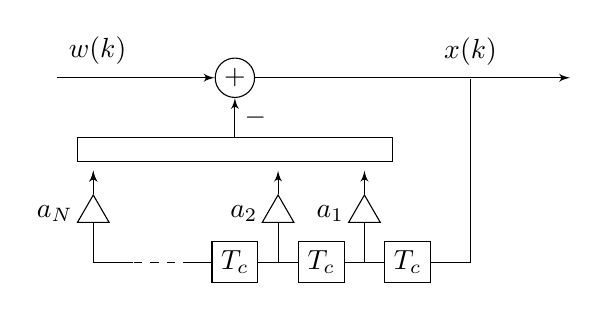
\begin{tikzpicture}[auto,>=latex']
\tikzstyle{block} = [draw, rectangle, minimum height=1cm, minimum width=1cm]

\node [coordinate, label={[label distance=0.05cm]60:$w(k)$}] (start) {};
\node [draw, circle,minimum size=0.5cm,inner sep=0pt, right = 2cm of start] (sum){$+$};
\node [draw, rectangle, minimum height=0.3cm, minimum width=4cm, below = 0.5cm of sum] (sum2){};
\node [coordinate, right = 4cm of sum] (end){};
\node [draw, rectangle, minimum height=0.5cm, minimum width=0.5cm, below = 1cm of sum2] (tc3){$T_c$};
\node [draw, rectangle, minimum height=0.5cm, minimum width=0.5cm, right = 0.5cm of tc3] (tc2){$T_c$};
\node [draw, rectangle, minimum height=0.5cm, minimum width=0.5cm, right = 0.5cm of tc2] (tc1){$T_c$};
\node [coordinate, right = 0.5cm of tc1] (aa){};
\node [coordinate, above = 2.33cm of aa, label={[label distance=0.05cm]90:$x(k)$}] (bb){};

\node [coordinate, left = 0.25cm of tc1] (a1){};
\node [coordinate, left = 0.25cm of tc2] (a2){};
\node [coordinate, left = 0.25cm of tc3] (a3){};
\node [coordinate, left = 1.5cm of tc3] (aN){};
\node [coordinate, right = 0.5cm of aN] (tN){};

\node[draw, regular polygon, regular polygon sides=3, scale=0.7, label=left:{$a_1$}, above = 0.5cm of a1] (gain1){};
\node[draw, regular polygon, regular polygon sides=3, scale=0.7, label=left:{$a_2$}, above = 0.5cm of a2] (gain2){};
\node[draw, regular polygon, regular polygon sides=3, scale=0.7, label=left:{$a_N$}, above = 0.5cm of aN] (gainN){};

\node [coordinate, above = 0.3cm of gain1] (b1){};
\node [coordinate, above = 0.3cm of gain2] (b2){};
\node [coordinate, above = 0.3cm of gainN] (bN){};

\draw [->] (start) --node[]{} (sum);
\draw [->] (sum2) --node[label=right:{$-$}]{} (sum);
\draw [->] (sum) --node{} (end);
\draw [-] (tc1) --node{} (tc2);
\draw [-] (tc2) --node{} (tc3);
\draw [-] (aN) --node{} (tN);
\draw [-] (tc1) --node{} (aa);
\draw [-] (aa) --node{} (bb);
\draw [-] (aa) --node{} (bb);
\draw [-] (a1) --node{} (gain1);
\draw [-] (a2) --node{} (gain2);
\draw [-] (aN) --node{} (gainN);
\draw [-] (tc3) --node{} (a3);
\draw [->] (gain1) --node{} (b1);
\draw [->] (gain2) --node{} (b2);
\draw [->] (gainN) --node{} (bN);
\draw [->] (gainN) --node{} (bN);
\draw [dashed] (a3) --node{} (tN);
\end{tikzpicture}
\caption{AR model}
\label{fig:armodel}
\end{figure}

The z-transform of the autocorrelation sequence of $x$ is given by
\begin{equation}
	P_x(z) = \frac{\sigma_w^2}{A(z) A^{*} \left( \frac{1}{z^{*}} \right) }
\end{equation}
hence the PSD of $x$ is the Fourier transform of $P_x(z)$:
\begin{equation}
	\mathcal{P}_x(f) = P_z(e^{j 2 \pi f T_c})= \frac{T_c \sigma_w^2}{|\mathcal{A}(f)|^2}
\end{equation}

The coefficients $a_1, a_2, ..., a_N$ can be computed using the Yule-Walker equations. Given the autocorrelation matrix
\begin{equation}
\mathbf{R} =
\begin{bmatrix}
\mathtt{r}_x(0)		&	\mathtt{r}_x(-1) 	& \cdots &	\mathtt{r}_x(-N+1) \\
\mathtt{r}_x(1)		&	\mathtt{r}_z(0)  	& \cdots &	\mathtt{r}_x(-N+2) \\
\vdots				&	\vdots        		& \vdots &	\vdots \\
\mathtt{r}_x(N-1)	&	\mathtt{r}_x(N-2)	& \cdots &	\mathtt{r}_x(0)
\end{bmatrix}
\end{equation}
and $ \mathbf{r} = [\mathtt{r}_x(1),  \mathtt{r}_x(2),  \mathtt{r}_x(N)]^T $, the vector $\mathbf{a}$ of the coefficients of the AR model is given by
\begin{equation}\label{eq:yulewalker}
	\mathbf{R} \, \mathbf{a} = - \mathbf{r}
\end{equation}
If $\mathbf{R}$ admits inverse (matrix is not ill conditioned), we obtain
\begin{equation}
	\mathbf{a} = -\mathbf{R}^{-1} \, \mathbf{r}
\end{equation}
The variance $\sigma_w ^2$ of the white noise $w(k)$ is then
\begin{equation}
	\sigma_w ^2 = \mathtt{r}_x(0) + \mathbf{r}^H \mathbf{a}
\end{equation}

To choose the parameter $N$ we decided to analyze the behavior of the cost function $J_{min} = \mathtt{r}_x(0) + \mathbf{r}_n^H \mathbf{a}$ in function of the number $N$ (from $1$ to $20$) of the coefficients.

\begin{figure}[H]
	\centering
	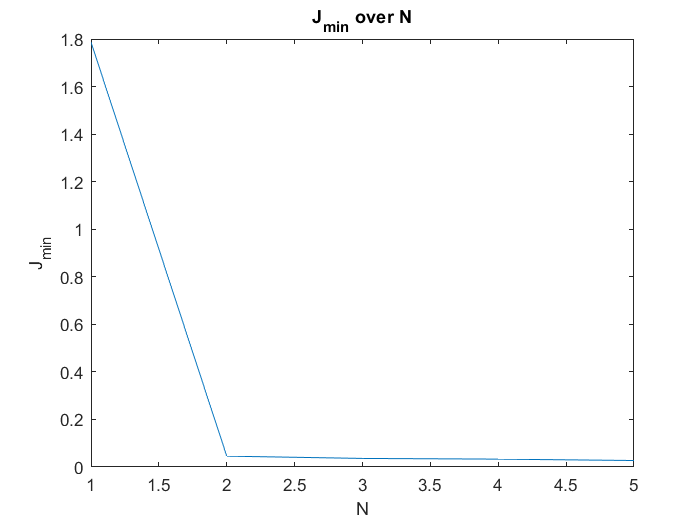
\includegraphics[width=0.5\textwidth]{choiceofn}
	\caption{$J_{min}$ over $N$}
	\label{fig:choiceofn}
\end{figure}

From Figure \ref{fig:choiceofn} it can be seen that a suitable choice is $N=2$.\\
Using this value the autocorrelation matrix $\mathbf{R}$ is indeed well conditioned, hence the solution is acceptable.

\subsection*{Results}
In Figure REF it is shown the power spectral density estimation using the methods described above, along with its actual value.

\section*{Problem 2}

\subsection*{Input signal}
In this case the input signal is the same as Section 1, except for the noise variance which now is $\sigma_w^2 = 2$.

\subsection*{Results}
In Figure REF it is shown the power spectral density estimation using the same methods of Problem 1, along with its actual value.

\section*{Problem 3}
The coefficients for the optimal error predictor are given by $ \mathbf{c} = -\mathbf{a}$, where the vector $\mathbf{a}$ is given by the coefficients of the AR model.

\begin{figure}[H]
	\centering
	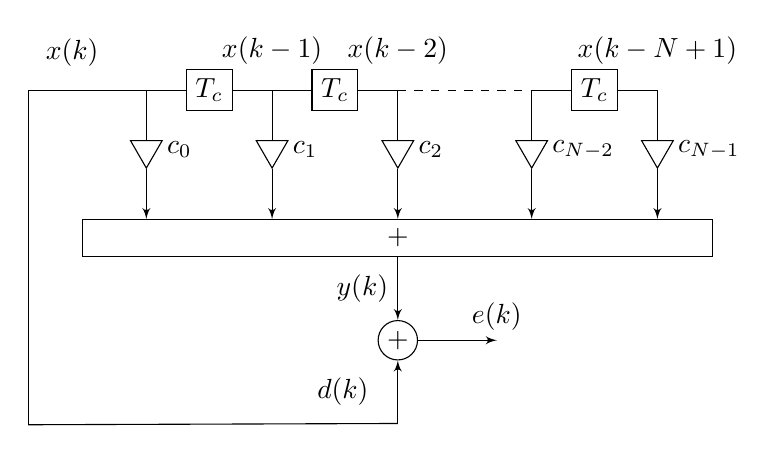
\begin{tikzpicture}[auto,>=latex']
	\tikzstyle{block} = [draw, rectangle, minimum height=1cm, minimum width=1cm]
	
	\node [coordinate, label={[label distance=0.2cm]60:$x(k)$}] (start) {};
	
	\node [draw, rectangle, minimum height=0.5cm, minimum width=0.5cm, right = 2cm of start] (tc1){$T_c$};
	\node [coordinate, left = 0.5cm of tc1] (m1){};
	
	\node[draw, regular polygon, regular polygon sides=3, rotate = 180, scale=0.7, label=left:{$c_0$}, below = 1cm of m1] (c0){};
	
	\node [coordinate, right = 0.5cm of tc1, label={[label distance=0.2cm]90:$x(k-1)$}] (m2){};
	\node[draw, regular polygon, regular polygon sides=3, rotate = 180, scale=0.7, label=left:{$c_1$}, below = 1cm of m2] (c1){};
	
	\node [draw, rectangle, minimum height=0.5cm, minimum width=0.5cm, right = 1cm of tc1] (tc2){$T_c$};

	\node [coordinate, right = 0.5cm of tc2, label={[label distance=0.2cm]90:$x(k-2)$}] (m3){};
	\node[draw, regular polygon, regular polygon sides=3, rotate = 180, scale=0.7, label=left:{$c_2$}, below = 1cm of m3] (c2){};
		
	\node [coordinate, right = 1.7cm of m3] (mN2){};
	\node[draw, regular polygon, regular polygon sides=3, rotate = 180, scale=0.7, label=left:{$c_{N-2}$}, below = 1cm of mN2] (cN2){};	
	
	\node [draw, rectangle, minimum height=0.5cm, minimum width=0.5cm, right = 0.5cm of mN2] (tcN1){$T_c$};
	\node [coordinate, right = 0.5cm of tcN1, label={[label distance=0.2cm]90:$x(k-N+1)$}] (mN1){};
	\node[draw, regular polygon, regular polygon sides=3, rotate = 180, scale=0.7, label=left:{$c_{N-1}$}, below = 1cm of mN1] (cN1){};
	
	\node [draw, rectangle, minimum height=0.3cm, minimum width=8cm, below = 1cm of c2] (sum){$+$};
	
	\node [draw, circle,minimum size=0.5cm,inner sep=0pt, below = 0.8cm of sum] (sum2){$+$};
	
	\node [coordinate, below = 0.8cm of sum2] (d1){};
	
	\node [coordinate, below = 1cm of c0] (v0){};
	\node [coordinate, below = 1cm of c1] (v1){};
	\node [coordinate, below = 1cm of c2] (v2){};
	\node [coordinate, below = 1cm of cN2] (vN2){};
	\node [coordinate, below = 1cm of cN1] (vN1){};
	
	\node [coordinate, below = 4.25cm of start] (d2){};
	
	\node [coordinate, right = 1cm of sum2, label=above:{$e(k)$}] (end){};
	
	\draw [-] (start) --node[]{} (tc1);
	\draw [-] (m1) --node[]{} (c0);
	\draw [-] (tc1) --node[]{} (tc2);
	\draw [-] (m2) --node[]{} (c1);
	\draw [-] (tc2) --node[]{} (m3);
	\draw [-] (m3) --node[]{} (c2);
	\draw [dashed] (m3) --node[]{} (mN2);
	\draw [-] (mN2) --node[]{} (cN2);
	\draw [-] (mN2) --node[]{} (tcN1);
	\draw [-] (tcN1) --node[]{} (mN1);
	\draw [-] (mN1) --node[]{} (cN1);
	\draw [->] (c0) --node[]{} (v0);
	\draw [->] (c1) --node[]{} (v1);
	\draw [->] (c2) --node[]{} (v2);
	\draw [->] (cN2) --node[]{} (vN2);
	\draw [->] (cN1) --node[]{} (vN1);
	\draw [->] (sum) --node[label=left:{$y(k)$}]{} (sum2);
	\draw [->] (d1) --node[label=left:{$d(k)$}]{} (sum2);
	\draw [-] (start) --node[]{} (d2);
	\draw [-] (d2) --node[]{} (d1);
	\draw [->] (sum2) --node[]{} (end);
	
	\end{tikzpicture}
	\caption{Wiener filter}
	\label{fig:wiener}
\end{figure}


\begin{figure}[H]
	\centering
	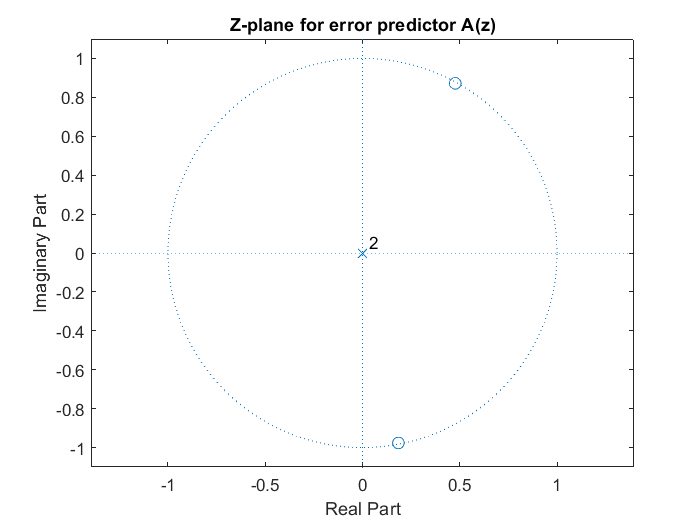
\includegraphics[width=0.5\textwidth]{zplane}
	\caption{Z-plane for the error predictor A(z)}
	\label{fig:zpln}
\end{figure}

As we can see in Figure \ref{fig:zpln}, the presence of zeros close the unit circle is a rough indicator of ``discrete'' frequency components.\\
The phase (normalized over $2 \pi$) of those zeros does determine the frequency of the discrete component.\\
In Table \ref{tab:errpred} the zeros of the transfer function $A(z)$ are reported, along with their magnitude and phase.


\begin{table}[H]
\centering
\begin{tabular}{ccccc}
\toprule
$z$		& $\Re[z]$ 	& $\Im[z]$			& $|z|$			& $f$ \\
\midrule
$z_1$ 	& 0.4766	& 0.8718			& 0.9936		& 0.1704 \\
$z_2$	& 0.1845	& -0.9762			& 0.9936		& 0.7797 \\
\bottomrule
\end{tabular}
\caption{Zeros of A(z)}
\label{tab:errpred}
\end{table}


\section*{Problem 4}

\subsection*{Least Mean-Square algorithm}
Given a signal $x(k)$, wide sense stationary, with zero mean, let $\mathbf{x}^T(k-1)$ be the vector $[x(k-1), x(k-2), \dots, x(k-N)]$. The one-step predictor of order $N$ tries to estimate the value of $x(k)$ given $\mathbf{x}^T(k-1)$.\\
This problem can be solved considering $\mathbf{x}^T(k-1)$ the input of a Wiener filter of order N and $x(k)$ the reference signal. Then the Wiener-Hopf equation computes the optimal coefficients of the filter with
\begin{equation}
	\mathbf{R} \mathbf{c}_{opt} = \mathbf{r}
\end{equation}
The LMS algorithm is a version of the steepest descent algorithm which provides an iterative method to approximate the optimal Wiener-Hopf solution, without knowing the autocorrelation matrix $\mathbf{R}$ and the vector $\mathbf{r}$.\\
The LMS algorithm updates the coefficients of the Wiener filter at each iteration $k$ with the equation
\begin{equation}\label{eq:lms-ue}
	\mathbf{c}(k+1) = \mathbf{c}(k) + \mu e(k) \mathbf{x}^*(k-1)
\end{equation}
where $e(k)$ is the estimation error between the reference signal $x(k)$ and the filter prediction $y(k)$.\\
Besides the filter order $N$, LMS relies on the update coefficient: $\mu = \frac{\tilde{\mu}}{N r_x(0)}$.\\
For convergence, it must hold $0 < \tilde{\mu} < 2$.\\
At each step, the algorithm computes $ y(k) = \mathbf{x}^T(k-1) \mathbf{c}(k)$ and $e(k)$, then it updates the coefficients using Equation (\ref{eq:lms-ue}).

\subsection*{Implementation and results}
At the beginning, we decided to initialize the Wiener filter coefficients to zero and the input signal before $k=0$ to zero: $\mathbf{c}(0) = \mathbf{0}$, $x(k) = 0, \forall \, k<0$. \\
Applying the algorithm on a single realization of the process we obtained a grassy behavior of the coefficients and the error.\\
Using $k_{max} = 800$ iterations and update coefficient $\tilde{\mu} = 0.05$ resulted in convergence even before reaching $k_{max}$.\\
Then we applied the LMS over 300 different realizations of the signal and took the average value for coefficients and error for each iteration. The behavior is much smoother than in the previous analysis, especially for $|e(k)|^2$.\\
In Table \ref{tab:predopt} are reported the coefficients of the predictor at convergence and their optimal value,computed using (\ref{eq:yulewalker}):

\begin{table}[H]
	\centering
	\begin{tabular}{c|cc|c|cc|c}
	\toprule
	Coefficient	& $\Re[c_{predictor}]$ 	& $\Re[c_{opt}]$	& Difference ($\%$)	& $\Im[c_{predictor}]$	& $\Im[c_{opt}]$ & Difference ($\%$) \\
	\midrule
	$c_1$ 	& 0.6612	& 0.6650			& 0.57 & -0.1045		& -0.1008 & 3.67 \\
	$c_2$	& -0.9390	& -0.9416			& 0.27 & 0.3045		& 0.3055 & 0.03 \\
	\bottomrule
	\end{tabular}
	\caption{Prediction and optimal coefficients}
	\label{tab:predopt}
\end{table}

In Figure \ref{fig:coeff1} it is shown the behavior of the coefficients $c_i, \, i=1,2$,  their mean across 300 realizations (as $k$ increases) and the optimal solution by the Wiener-Hopf equation.\\
In Figure \ref{fig:err300} it is shown the behavior of the cost function $J(k) = E \left[ |e(k)|^2 \right]$  across 300 realizations and its optimal solution $J_{min}$, as the number of iterations $k$ increases.

\begin{figure}[H]
	\centering
	\subfloat[Real and imaginary part of $c_1$]{
		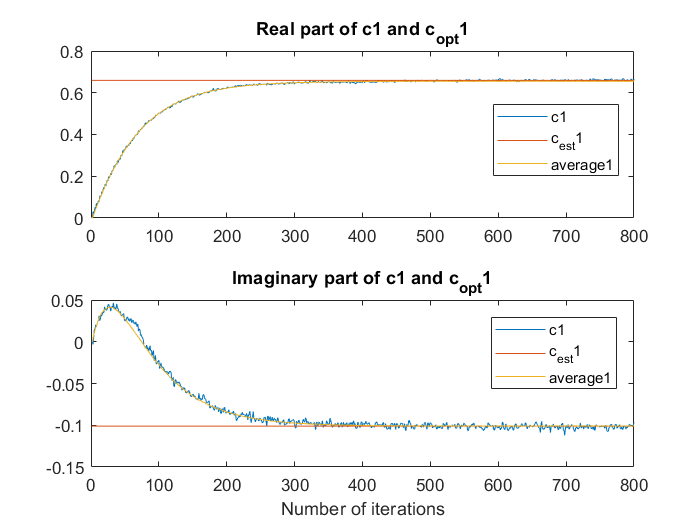
\includegraphics[width=0.5\textwidth]{c1_1real}}
	\subfloat[Real and imaginary part of $c_2$]{
	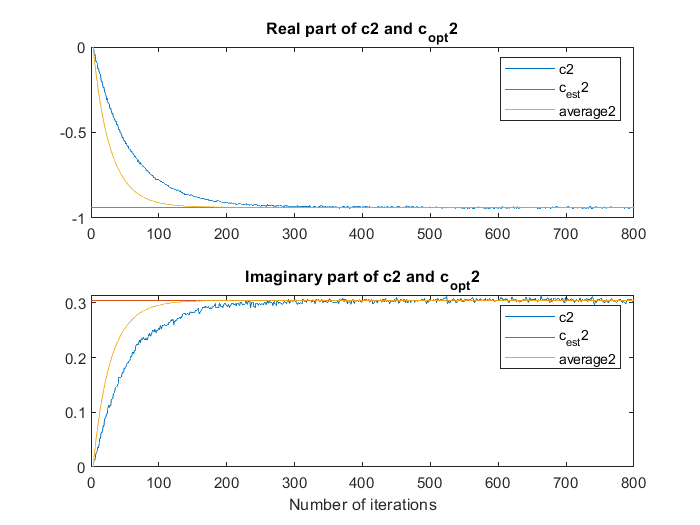
\includegraphics[width=0.5\textwidth]{c2_1real}}
	\caption{Coefficients for one realization}
	\label{fig:coeff1}
\end{figure}

\iffalse
%Useless figure
\begin{figure}[H]
	\centering
	\subfloat[Real and imaginary part of $c_1$]{
		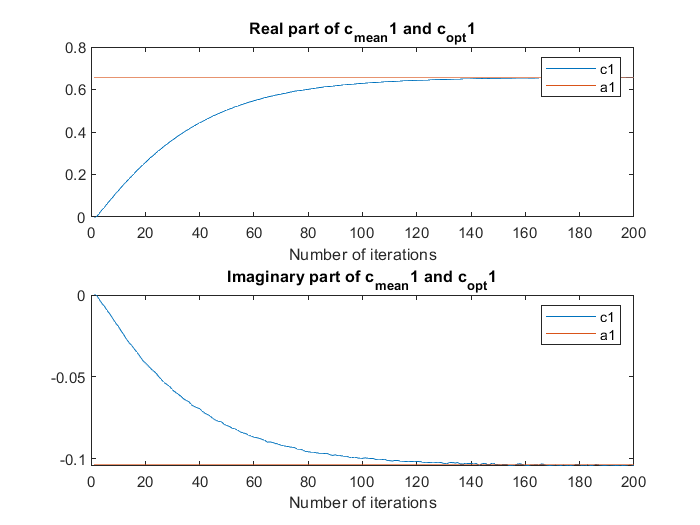
\includegraphics[width=0.5\textwidth]{c1_300real}}
	\subfloat[Real and imaginary part of $c_2$]{
		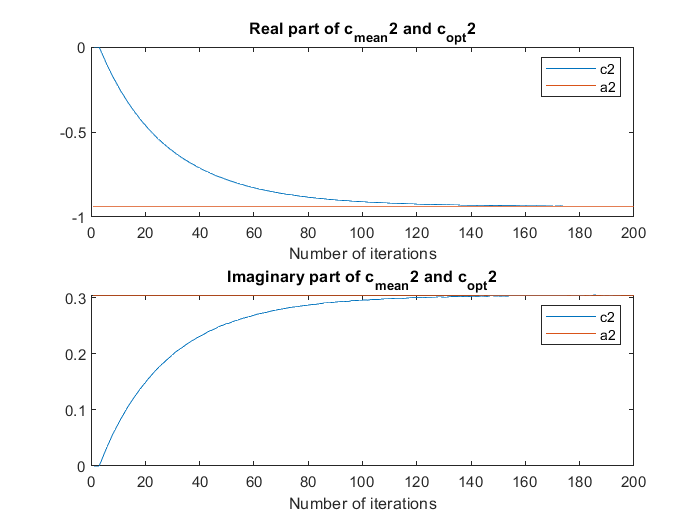
\includegraphics[width=0.5\textwidth]{c2_300real}}
	\caption{Coefficients by averaging over 300 realizations}
	\label{fig:coeff300}
\end{figure}
\fi

\begin{figure}[H]
	\centering
	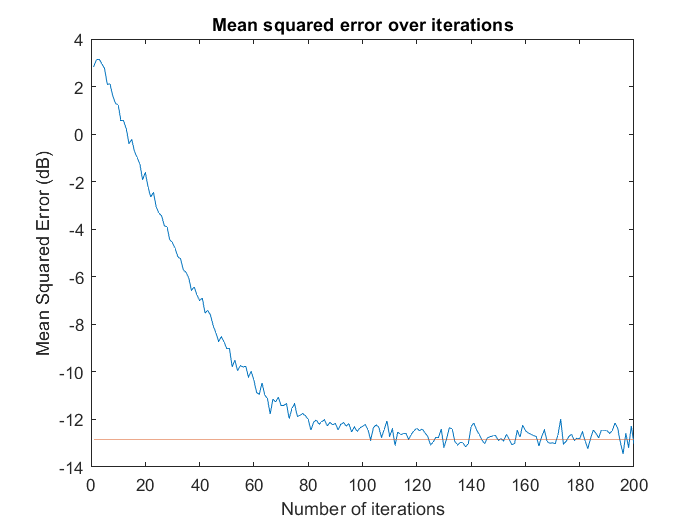
\includegraphics[width=0.5\textwidth]{error_300real}
	\caption{Mean squared error by averaging over 300 realizations}
	\label{fig:err300}
\end{figure}

\begin{thebibliography}{15}
	\bibitem{nevio<3}
	Nevio Benvenuto, Giovanni Cherubini,
	\textit{Algorithms for Communication Systems and their Applications}. 
	Wiley, 2002.
\end{thebibliography}

\end{document}